\documentclass[11pt,letterpaper]{article}

\usepackage[utf8]{inputenc}
\usepackage[T1]{fontenc}
\usepackage[spanish,es-nodecimaldot]{babel}
\usepackage[letterpaper,margin=2.25cm,headheight=15pt]{geometry}
\usepackage[protrusion=true,expansion=false]{microtype}
\usepackage{xcolor}
\usepackage{graphicx}
\usepackage{booktabs}
\usepackage{tabularx}
\usepackage{longtable}
\usepackage{array}
\usepackage{enumitem}
\usepackage{fancyhdr}
\usepackage{hyperref}
\usepackage{xurl}
\usepackage{listings}
\usepackage{float}

\ifdefined\pdfinfoomitdate\pdfinfoomitdate=1\fi
\ifdefined\pdftrailerid\pdftrailerid{}\fi
\ifdefined\pdfsuppressptexinfo\pdfsuppressptexinfo=15\fi

\definecolor{ugblue}{HTML}{006A8D}
\definecolor{deepgreen}{HTML}{123D3A}
\definecolor{softgray}{HTML}{F1F5F4}
\definecolor{midgray}{HTML}{5D6B6B}
\definecolor{warning}{HTML}{A45A00}

\hypersetup{
  colorlinks=true,
  linkcolor=ugblue,
  urlcolor=ugblue,
  hypertexnames=false,
  pdftitle={Informe del Sprint 1 - Ambiente reproducible y DevOps},
  pdfauthor={Emily Dayan Robles Alvarado y Lesly Samay Velasquez Anchundia}
}

\pagestyle{fancy}
\fancyhf{}
\lhead{Informe del Sprint 1}
\rhead{Prototipo BI asistido por IA}
\cfoot{\thepage}

\setlength{\parindent}{0pt}
\setlength{\parskip}{0.55em}
\setlist[itemize]{leftmargin=1.5em,itemsep=0.25em,topsep=0.3em}
\setlist[enumerate]{leftmargin=1.7em,itemsep=0.35em,topsep=0.35em}
\renewcommand{\arraystretch}{1.22}
\newcommand{\statusok}{\textcolor{deepgreen}{\textbf{Completado}}}
\newcommand{\statusnext}{\textcolor{warning}{\textbf{Siguiente sprint}}}
\newcommand{\file}[1]{\texttt{#1}}

\lstdefinestyle{terminal}{
  basicstyle=\ttfamily\small,
  backgroundcolor=\color{softgray},
  frame=single,
  rulecolor=\color{midgray},
  breaklines=true,
  columns=fullflexible,
  keepspaces=true,
  showstringspaces=false,
  xleftmargin=0.4em,
  xrightmargin=0.4em,
  aboveskip=0.6em,
  belowskip=0.6em
}

\begin{document}
\hypersetup{pageanchor=false}

\begin{titlepage}
  \thispagestyle{empty}
  \vspace*{0.8cm}
  {\color{ugblue}\rule{\textwidth}{2.8pt}}
  \vspace{1.2cm}

  {\Large Universidad de Guayaquil\\[0.25em]
  Facultad de Ciencias Matemáticas y Físicas\\
  Carrera de Software}

  \vfill

  {\color{deepgreen}\fontsize{30}{35}\selectfont\textbf{Informe del Sprint 1}}\\[0.7em]
  {\LARGE Ambiente reproducible, repositorio y DevOps}\\[0.6em]
  {\large Prototipo web de inteligencia de negocios asistido por IA}

  \vspace{1.5cm}

  \begin{tabularx}{\textwidth}{@{}>{\bfseries}l X@{}}
    Autoras & Emily Dayan Robles Alvarado y Lesly Samay Velásquez Anchundia \\
    Identificador & SPR-01 \\
    Fecha de ejecución & 24 de agosto al 2 de septiembre de 2026 \\
    Repositorio & \href{https://github.com/LFXAS/prototipo-bi-ia}{LFXAS/prototipo-bi-ia} \\
    Línea base & Cierre aprobado e integrado mediante PR \#15 y PR \#16 \\
    Estado & \statusok \\
  \end{tabularx}

  \vfill
  {\color{ugblue}\rule{\textwidth}{2.8pt}}
\end{titlepage}

\hypersetup{pageanchor=true}
\pagenumbering{roman}
\tableofcontents
\newpage
\pagenumbering{arabic}

\section{Resumen ejecutivo}

El trabajo realizado puede registrarse como el \textbf{Sprint 1} del proyecto. Produjo un incremento técnico terminado, verificable y reutilizable: el repositorio público con escritura controlada, el entorno Docker autocontenido, la aplicación base React/FastAPI, PostgreSQL, SQL Server con AdventureWorks, automatización de pruebas, CI/CD, publicación de imágenes y documentación reproducible.

El objetivo deliberado de este sprint fue reducir el riesgo tecnológico antes de desarrollar funcionalidades de negocio. Por ello, no se implementaron todavía autenticación, ETL, KPIs, copiloto con IA ni pronóstico. El módulo de seguridad RBAC quedó previsto mediante límites modulares y reglas arquitectónicas, tal como exige el alcance académico.

La denominación Sprint 1 es válida porque existieron un objetivo acotado, un conjunto priorizado de elementos de trabajo, criterios de aceptación, un incremento ejecutable, revisión mediante evidencias y una retrospectiva. Este informe formaliza dichas actividades para su incorporación en la tesis; no pretende afirmar ceremonias o métricas que no se hayan observado.

\section{Ficha del sprint}

\begin{tabularx}{\textwidth}{@{}>{\bfseries}p{0.27\textwidth}X@{}}
  \toprule
  Campo & Definición \\
  \midrule
  Nombre & Base reproducible y canal DevOps \\
  Objetivo & Dejar el entorno completo ejecutándose desde cero con Docker y publicarlo de forma controlada y repetible. \\
  Resultado esperado & Una persona autorizada puede clonar el repositorio, configurar secretos locales y levantar el mismo ambiente sin instalar Python, Node.js ni motores de base de datos en el host. \\
  Alcance funcional & Salud técnica y pantalla de estado; sin módulos de negocio. \\
  Fuente externa & SQL Server con AdventureWorks 2022, accesible mediante un usuario de sólo lectura. \\
  Datos internos & PostgreSQL con esquemas iniciales \file{app} y \file{mart}. \\
  Automatización & Docker Compose, Make, scripts, GitHub Actions y GitHub Container Registry. \\
  Definición de terminado & Construcción limpia, pruebas aprobadas, cuatro servicios saludables, restauración verificable, documentación compilada y CI/CD exitosa. \\
  \bottomrule
\end{tabularx}

\section{Relación con el anteproyecto}

El anteproyecto corregido plantea una prueba de concepto con una fuente SQL Server/AdventureWorks, generación asistida por IA, aprobación humana, ETL hacia PostgreSQL, cinco KPIs, tres visualizaciones, insights explicables y un pronóstico mensual por regresión lineal evaluado con MAPE y RMSE.

El Sprint 1 no adelanta estas funciones. Establece la plataforma necesaria para implementarlas con trazabilidad y separación de responsabilidades. También incorpora el requerimiento institucional de un módulo de seguridad, conservándolo como arquitectura pendiente y no como funcionalidad simulada.

\begin{tabularx}{\textwidth}{@{}X X l@{}}
  \toprule
  Necesidad del proyecto & Aporte del Sprint 1 & Estado \\
  \midrule
  Fuente SQL Server & Contenedor aislado y restauración automática de AdventureWorks 2022 & \statusok \\
  Lectura controlada & Usuario \file{bi\_reader}, intención de lectura y denegación de escritura & \statusok \\
  Datamart PostgreSQL & Instancia propia y esquemas \file{app}/\file{mart} & \statusok \\
  Aplicación web & React + TypeScript y API FastAPI conectados & \statusok \\
  Seguridad RBAC & Paquete, entidades previstas y reglas de autorización documentadas & \statusnext \\
  Módulos BI e IA & Límites de módulos definidos, sin lógica funcional & \statusnext \\
  Reproducibilidad & Docker, scripts, guía, imágenes y controles automáticos & \statusok \\
  \bottomrule
\end{tabularx}

\section{Backlog ejecutado}

\begin{longtable}{@{}p{0.10\textwidth}p{0.27\textwidth}p{0.40\textwidth}p{0.08\textwidth}@{}}
  \toprule
  \textbf{ID} & \textbf{Elemento} & \textbf{Criterio de aceptación} & \textbf{Estado} \\
  \midrule
  \endfirsthead
  \toprule
  \textbf{ID} & \textbf{Elemento} & \textbf{Criterio de aceptación} & \textbf{Estado} \\
  \midrule
  \endhead
  SP1-01 & Revisar el anteproyecto & Alcance incluido, exclusiones y límite de la fase documentados. & Hecho \\
  SP1-02 & Crear estructura del repositorio & Frontend, backend, infraestructura, documentación y automatización separados. & Hecho \\
  SP1-03 & Dockerizar FastAPI & Imagen de desarrollo, prueba y producción; endpoint de salud accesible. & Hecho \\
  SP1-04 & Dockerizar React/Vite & Recarga en desarrollo, prueba automatizada y Nginx en producción. & Hecho \\
  SP1-05 & Aislar PostgreSQL & Volumen propio, salud y esquemas iniciales sin tocar otras instancias. & Hecho \\
  SP1-06 & Aislar SQL Server & Volumen propio, restauración idempotente de AdventureWorks y usuario lector. & Hecho \\
  SP1-07 & Orquestar el conjunto & \file{docker compose up --build -d} inicia los cuatro servicios. & Hecho \\
  SP1-08 & Automatizar operación & \file{make bootstrap}, pruebas, validación y diagnóstico disponibles. & Hecho \\
  SP1-09 & Configurar Git/GitHub & Rama \file{main}, remoto privado y convenciones de contribución. & Hecho \\
  SP1-10 & Implementar CI/CD & Pruebas en cada cambio y publicación de cinco imágenes en GHCR. & Hecho \\
  SP1-11 & Documentar réplica & Otra máquina puede levantar por código o imágenes publicadas. & Hecho \\
  SP1-12 & Mantener trazabilidad & Bitácora LaTeX/PDF versionada y compilada automáticamente. & Hecho \\
  \bottomrule
\end{longtable}

\section{Arquitectura entregada}

\begin{center}
\fcolorbox{ugblue}{softgray}{%
  \begin{minipage}{0.90\textwidth}
    \centering
    \textbf{Navegador}\\[0.25em]
    $\downarrow$\\[0.25em]
    \textbf{React + Vite} (desarrollo) / \textbf{Nginx} (producción)\\[0.25em]
    $\downarrow$ HTTP/JSON\\[0.25em]
    \textbf{FastAPI}\\[0.3em]
    \begin{tabular}{c@{\hspace{2cm}}c}
      $\swarrow$ & $\searrow$ \\
      \textbf{PostgreSQL} & \textbf{SQL Server} \\
      interno y datamart & AdventureWorks de sólo lectura
    \end{tabular}
  \end{minipage}}
\end{center}

Los servicios comparten únicamente la red creada por Compose. Los puertos de PostgreSQL y SQL Server se publican como 55432 y 51433, respectivamente, para evitar colisiones con las instancias habituales 5432 y 1433 del equipo anfitrión. Los volúmenes pertenecen exclusivamente al proyecto \file{bi-ia-prototype}.

FastAPI organiza los límites futuros en \file{security}, \file{parameters}, \file{metadata}, \file{copilot}, \file{etl}, \file{analytics}, \file{forecasting} y \file{reports}. Sólo el módulo \file{system} contiene comportamiento durante este sprint.

\section{Procedimiento ejecutado paso a paso}

\subsection{Revisión y congelación del alcance}

Se inspeccionaron las once páginas del anteproyecto. Se separaron las capacidades finales del prototipo de las tareas permitidas en la primera fase. El resultado se registró en \file{docs/scope.md}; la decisión principal fue no implementar módulos de negocio mientras el entorno no estuviera reproducible.

\subsection{Definición del enfoque Docker-first}

Se adoptó Docker como única dependencia de ejecución del equipo anfitrión. La decisión quedó registrada en \file{docs/decisions/0001-docker-first.md}. Cada componente propio posee un Dockerfile con una etapa acorde a desarrollo, pruebas o producción.

\subsection{Creación del backend}

Se creó una aplicación FastAPI con configuración mediante variables de entorno, enrutamiento versionado, conexión inicial a PostgreSQL, soporte de Alembic y pruebas. Se añadieron dos controles:

\begin{itemize}
  \item \file{/api/v1/health/live}: confirma que el proceso de la API responde;
  \item \file{/api/v1/health/ready}: confirma además la conexión con PostgreSQL.
\end{itemize}

\subsection{Creación del frontend}

Se creó React con Vite y TypeScript. La pantalla técnica consulta el backend y presenta el estado de la API, los componentes disponibles y los módulos deliberadamente pendientes. En producción, Nginx sirve los archivos estáticos y redirige \file{/api/} al backend.

\subsection{Preparación de PostgreSQL}

La imagen propia parte de PostgreSQL y ejecuta un script de inicialización que crea los esquemas \file{app} y \file{mart}. Las credenciales se inyectan desde \file{.env}; el archivo real está excluido de Git y sólo se publica \file{.env.example}.

\subsection{Preparación de SQL Server y AdventureWorks}

Se creó una imagen que arranca SQL Server, descarga el respaldo oficial \file{AdventureWorks2022.bak} cuando el volumen está vacío, restaura la base de forma idempotente y crea \file{bi\_reader}. La cuenta recibe capacidad de conexión y lectura, junto con denegaciones explícitas de escritura. La sonda de salud utiliza esa cuenta, no la cuenta administrativa.

\subsection{Orquestación aislada}

\file{compose.yaml} define los cuatro servicios, dependencias condicionadas por salud, red, puertos y volúmenes propios. El conjunto no referencia nombres ni volúmenes de contenedores preexistentes en el computador.

\begin{lstlisting}[style=terminal,language=bash]
cp .env.example .env
# Reemplazar cada valor ChangeMe_* antes de continuar.
make bootstrap
\end{lstlisting}

\subsection{Automatización de pruebas y operación}

Se añadieron \path{Makefile}, \path{scripts/bootstrap.sh}, \path{scripts/wait-for-stack.sh} y \path{scripts/verify-environment.sh}. Estos recursos construyen, esperan la restauración, comprueban salud y ejecutan controles de calidad sin instalar herramientas de desarrollo en el host.

\subsection{Inicialización de Git y publicación reproducible}

Se inicializó Git con \file{main}, se aplicó una política para excluir secretos y datos locales, y se creó el repositorio \href{https://github.com/LFXAS/prototipo-bi-ia}{LFXAS/prototipo-bi-ia}. Su visibilidad vigente es pública para facilitar la réplica académica, mientras que la escritura permanece restringida a colaboradoras autorizadas. Las contribuciones siguen Conventional Commits y una plantilla de pull request.

\subsection{Integración y entrega continuas}

CI valida Compose y construye las etapas de prueba de frontend, backend e infraestructura. CD vuelve a comprobar la entrega y publica cinco imágenes públicas en GHCR: frontend, backend, PostgreSQL, SQL Server y documentación. Las etiquetas incluyen rama, versión y SHA. CD publica imágenes, pero todavía no despliega automáticamente una VM Azure.

Los volúmenes no se publican. El estado se reconstruye desde scripts, migraciones y el respaldo oficial; esta decisión evita distribuir contraseñas o datos dependientes de una máquina.

\subsection{Documentación y trazabilidad}

Se crearon README, guía de réplica, descripción de arquitectura, ADR y bitácora LaTeX. El repositorio incluye reglas para que futuras sesiones de desarrollo actualicen pruebas y documentos antes de entregar cambios. Como cierre, se adoptó SDD para los sprints posteriores: una especificación versionada definirá cada capacidad funcional antes de su implementación.

\clearpage
\section{Trazabilidad técnica ampliada del incremento}

El incremento no se limita a que la pantalla responda. La trazabilidad conecta una necesidad del Sprint 1 con un archivo, un control automático y una evidencia observable.

\begin{longtable}{@{}p{0.20\textwidth}p{0.28\textwidth}p{0.23\textwidth}p{0.21\textwidth}@{}}
  \toprule
  \textbf{Necesidad} & \textbf{Implementación} & \textbf{Control} & \textbf{Evidencia} \\
  \midrule
  \endfirsthead
  \toprule
  \textbf{Necesidad} & \textbf{Implementación} & \textbf{Control} & \textbf{Evidencia} \\
  \midrule
  \endhead
  Repetibilidad & Dockerfiles, Compose y plantillas de entorno & \file{make compose-check} & Configuraciones interpretadas sin error \\
  Aislamiento & Nombre Compose, puertos y volúmenes propios & \file{docker compose ps} & Recursos prefijados por el proyecto \\
  Calidad backend & Etapa Docker \file{test} & Ruff, formato, Mypy y Pytest & Construcción exitosa en CI \\
  Calidad frontend & Etapa Docker \file{test} & ESLint, Vitest y Vite build & Construcción exitosa en CI \\
  Fuente lectora & Usuario \file{bi\_reader} y sonda real & Consulta permitida y escritura denegada & SQL Server saludable \\
  Persistencia & Volúmenes nombrados & Reinicio y recreación sin \file{--volumes} & Datos conservados \\
  Integración & PR hacia \file{develop} & Aprobación y controles obligatorios & PR \#15 fusionado \\
  Promoción & PR \file{develop} hacia \file{main} & Política de flujo y CI & PR \#16 fusionado \\
  Entrega & Workflow CD y GHCR & Verificación previa y matriz & Cinco imágenes publicadas \\
  Documentación & LaTeX dentro de Docker & Compilación y \file{git diff --exit-code} & Tres PDF versionados \\
  Réplica & Compose de desarrollo y de entrega & Prueba en VM Ubuntu & Aplicación levantada fuera del equipo principal \\
  Gobierno futuro & SDD, plantilla y especificaciones & Revisión antes del código & Contrato de Sprint 2 preparado \\
  \bottomrule
\end{longtable}

\section{Detalle del ciclo DevOps aplicado}

\subsection{Planificación y especificación}

El alcance se obtuvo del anteproyecto y se congeló en \file{docs/scope.md}. La decisión Docker-first se formalizó en un ADR. El Sprint 1 se ejecutó antes de adoptar formalmente SDD; como mejora de proceso, el cierre incorporó \file{docs/sdd-workflow.md}, una plantilla y la especificación preliminar del Sprint 2.

\subsection{Construcción y configuración}

\file{.env.example} documenta los valores de desarrollo sin secretos reales. \file{compose.yaml} construye servicios desde el código. \file{compose.prod.yaml} selecciona etapas estables durante una construcción local. \file{compose.release.yaml} descarga las imágenes publicadas y usa otros puertos y volúmenes. Esta separación permitió mantener simultáneamente un entorno editable y otro de comprobación.

\subsection{Integración continua}

El workflow \file{ci.yml} se activa en pushes y PR hacia \file{develop} o \file{main}. Sus trabajos validan el flujo de ramas, las variantes Compose, las etapas de prueba de FastAPI y React, las imágenes de infraestructura y los tres documentos. Los ejecutores son efímeros: al terminar no dejan servicios de desarrollo activos.

La protección de ramas agrega una aprobación humana a la verificación automática. CI puede detectar incumplimientos, pero no decide si el cambio satisface el objetivo académico; esa responsabilidad permanece en la revisión.

\subsection{Entrega continua}

El workflow \file{cd.yml} se activa al integrar en \file{main} o crear una etiqueta \file{v*}. Primero revalida backend, frontend y la configuración de entrega. Después una matriz construye y publica cinco imágenes en GHCR. Cada artefacto recibe una etiqueta de rama o versión y otra derivada del SHA del commit. El CD entregado no despliega Azure; ese alcance se mantiene explícitamente pendiente.

\subsection{Operación y retroalimentación}

Las sondas de salud, registros de Docker, estado de Actions, digest de imágenes y prueba de réplica forman el ciclo de retroalimentación. Los incidentes encontrados se transformaron en cambios versionados: corrección de salud IPv4, espera de recuperación de AdventureWorks, permisos efectivos del lector, caché LaTeX escribible y exclusión correcta de secretos.

\section{Archivos producidos y responsabilidad}

\begin{longtable}{@{}p{0.34\textwidth}p{0.58\textwidth}@{}}
  \toprule
  \textbf{Archivo o carpeta} & \textbf{Responsabilidad dentro del Sprint 1} \\
  \midrule
  \endfirsthead
  \toprule
  \textbf{Archivo o carpeta} & \textbf{Responsabilidad dentro del Sprint 1} \\
  \midrule
  \endhead
  \file{backend/Dockerfile} & Ambientes Python de desarrollo, prueba y producción; controlador ODBC y usuario no privilegiado. \\
  \file{frontend/Dockerfile} & Dependencias reproducibles, servidor Vite, controles y entrega Nginx. \\
  \file{infra/postgres/} & Imagen PostgreSQL e inicialización de los esquemas \file{app} y \file{mart}. \\
  \file{infra/sqlserver/} & SQL Server, restauración idempotente y cuenta de sólo lectura. \\
  \file{infra/docs/} & Compilador LaTeX versionado como imagen. \\
  \file{compose.yaml} & Desarrollo con recarga, bases locales y perfil de vista Nginx. \\
  \file{compose.prod.yaml} & Sobreescritura para etapas estables construidas localmente. \\
  \file{compose.release.yaml} & Entrega aislada que consume GHCR sin compilar. \\
  \file{Makefile} y \file{scripts/} & Interfaz operativa, esperas, verificación y política de ramas. \\
  \file{.github/workflows/ci.yml} & Integración continua sin permiso de publicación. \\
  \file{.github/workflows/cd.yml} & Verificación y publicación de cinco imágenes. \\
  \file{.github/dependabot.yml} & Propuestas semanales de mantenimiento de dependencias. \\
  \file{docs/} & Alcance, arquitectura, decisiones, réplica, SDD, manual, informe y bitácora. \\
  \bottomrule
\end{longtable}

\section{Validación manual equivalente}

La siguiente secuencia resume lo que el equipo ejecutó o automatizó para declarar terminado el incremento:

\begin{lstlisting}[style=terminal,language=bash]
cp .env.example .env
# Sustituir marcadores ChangeMe_*
docker compose config --quiet
docker compose --profile delivery config --quiet
docker compose --env-file .env.release.example \
  -f compose.release.yaml config --quiet
docker build --target test -t backend:test backend
docker build --target test -t frontend:test frontend
make docs
make bootstrap
docker compose ps
curl --fail http://localhost:8000/api/v1/health/ready
\end{lstlisting}

\section{Cierre real del Sprint 1}

El PR \#15 integró en \file{develop} el cierre documental y la adopción de SDD. El PR \#16 promovió \file{develop} a \file{main} con aprobación, controles satisfactorios y sin conflictos. Por ello, el estado del incremento es cerrado y promocionado; Azure, RBAC, parámetros y capacidades BI permanecen fuera de este sprint.


\section{Evidencias del incremento}

\subsection{Interfaz técnica}

La Figura~\ref{fig:frontend} muestra la pantalla ejecutándose en \file{localhost:5173}. La insignia verde confirma que el frontend pudo consultar la API. La interfaz declara de forma transparente qué módulos quedan para sprints posteriores.

\begin{figure}[H]
  \centering
  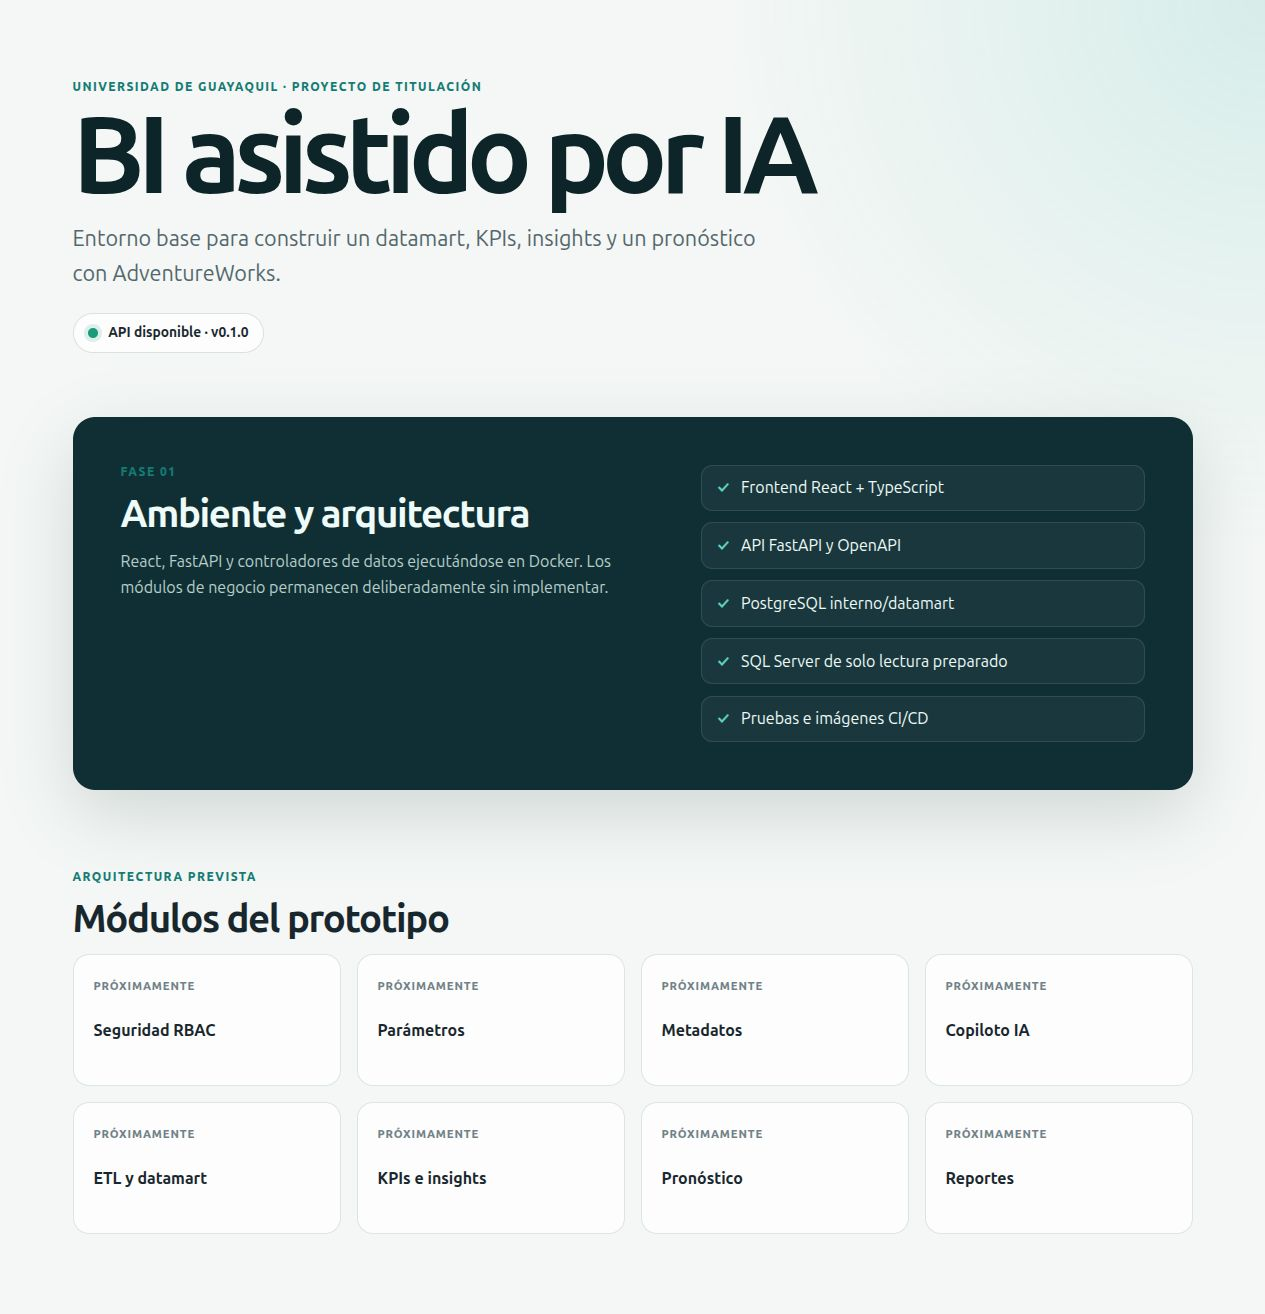
\includegraphics[width=0.88\textwidth]{../assets/sprint-01/frontend.jpg}
  \caption{Pantalla inicial del prototipo y estado del ambiente.}
  \label{fig:frontend}
\end{figure}

\subsection{Contrato de la API}

La documentación OpenAPI de la Figura~\ref{fig:openapi} presenta únicamente los endpoints técnicos habilitados en esta fase. Esta evidencia confirma el cumplimiento del límite del sprint: infraestructura funcional sin módulos de negocio prematuros.

\begin{figure}[H]
  \centering
  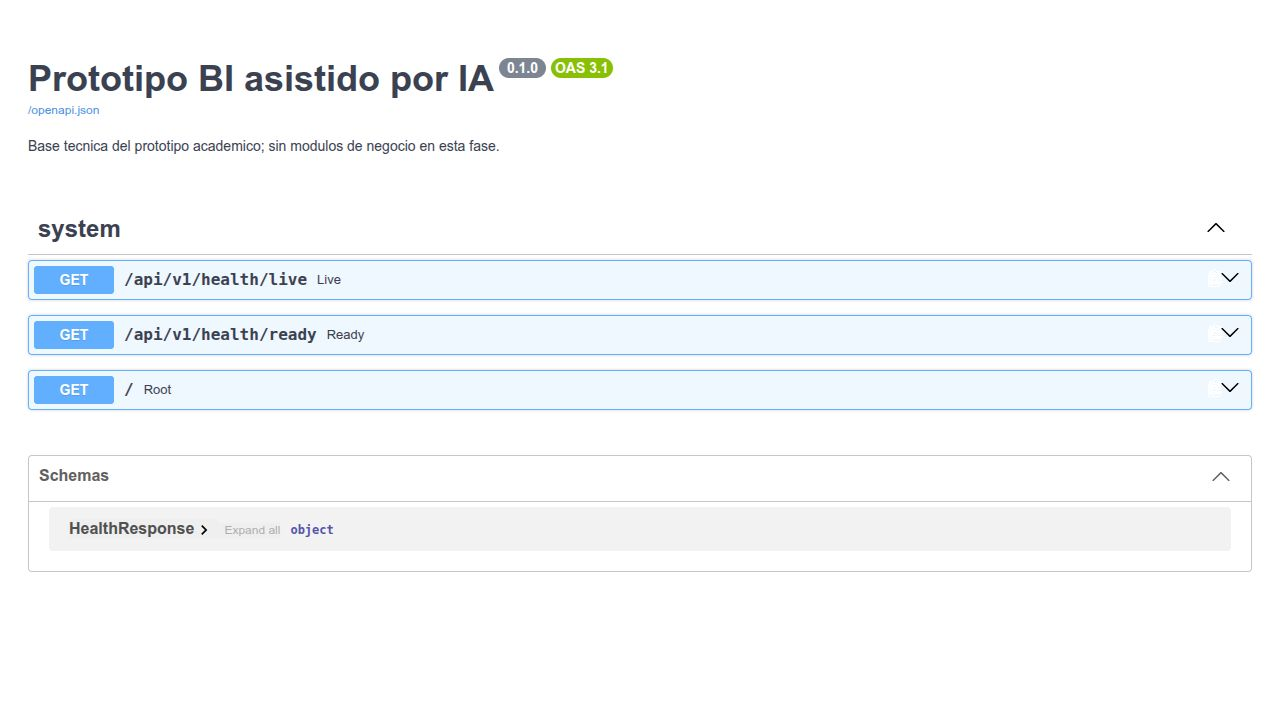
\includegraphics[width=\textwidth]{../assets/sprint-01/openapi.jpg}
  \caption{Documentación OpenAPI de FastAPI en \file{localhost:8000/docs}.}
  \label{fig:openapi}
\end{figure}

\subsection{Estado de los servicios}

\begin{tabularx}{\textwidth}{@{}l X l l@{}}
  \toprule
  Servicio & Función & Puerto anfitrión & Estado observado \\
  \midrule
  frontend & React/Vite y proxy a la API & 5173 & Saludable \\
  backend & FastAPI y OpenAPI & 8000 & Saludable \\
  postgres & Datos internos y futuro datamart & 55432 & Saludable \\
  sqlserver & AdventureWorks externo & 51433 & Saludable \\
  \bottomrule
\end{tabularx}

La respuesta del control de preparación fue:

\begin{lstlisting}[style=terminal]
{"status":"ok","service":"Prototipo BI asistido por IA",
 "version":"0.1.0","postgres":"ok"}
\end{lstlisting}

AdventureWorks fue reconstruida desde un volumen vacío. La verificación encontró 71 tablas. La cuenta \file{bi\_reader} pudo ejecutar \file{SELECT} y no pudo insertar, confirmando el control del motor y no sólo una opción de conexión.

\subsection{Pruebas y entrega continua}

\begin{tabularx}{\textwidth}{@{}X l X@{}}
  \toprule
  Control & Resultado & Evidencia \\
  \midrule
  Backend & Aprobado & Ruff, Mypy y dos pruebas Pytest en imagen Docker \\
  Frontend & Aprobado & ESLint, Vitest y build Vite en imagen Docker \\
  Compose & Aprobado & Variantes de desarrollo y publicación válidas \\
  Bitácora & Aprobado & PDF reproducible sin diferencias en CI \\
  CI & Éxito & \href{https://github.com/LFXAS/prototipo-bi-ia/actions/runs/32749237009}{Ejecución 32749237009} \\
  CD & Éxito & \href{https://github.com/LFXAS/prototipo-bi-ia/actions/runs/32749237059}{Ejecución 32749237059} \\
  GHCR & Publicado & Cinco imágenes públicas con etiquetas \file{main} y \file{sha-*} \\
  \bottomrule
\end{tabularx}

\section{Incidencias y resolución}

\begin{longtable}{@{}p{0.27\textwidth}p{0.33\textwidth}p{0.33\textwidth}@{}}
  \toprule
  \textbf{Incidencia} & \textbf{Diagnóstico} & \textbf{Resolución} \\
  \midrule
  \endfirsthead
  \toprule
  \textbf{Incidencia} & \textbf{Diagnóstico} & \textbf{Resolución} \\
  \midrule
  \endhead
  Caché npm sin escritura & La caché predeterminada estaba en una ubicación restringida. & Se generó el lockfile con una caché temporal controlada. \\
  Formato/import del backend & Las reglas vigentes de Ruff detectaron diferencias. & Se corrigió el código antes de congelar la imagen de prueba. \\
  Inicialización duplicada de pruebas & \file{jest-dom} se cargaba dos veces. & Se eliminó la importación redundante y Vitest pasó. \\
  Vulnerabilidades de npm & Las versiones iniciales de Vite/Vitest tenían avisos conocidos. & Se actualizaron a versiones corregidas; el lockfile quedó sin vulnerabilidades reportadas. \\
  Salud de frontend por IPv6 & BusyBox resolvía \file{localhost} por IPv6 y Vite atendía en IPv4. & La sonda cambió a \file{127.0.0.1}. \\
  Lector de SQL Server sin conexión & Una denegación amplia de \file{CONTROL} anuló un permiso subordinado. & Se retiró esa denegación y se mantuvieron denegaciones explícitas de escritura. \\
  Advertencias de Node.js en Actions & Varias acciones utilizaban una generación anterior del runtime. & Se actualizaron las acciones oficiales y se repitieron CI/CD con éxito. \\
  Invitaciones por correo pendientes & La API de colaboradores requiere nombres de usuario y los correos no devolvieron cuentas públicas. & Se aplazaron las invitaciones hasta disponer de los identificadores GitHub o una sesión web autenticada. \\
  \bottomrule
\end{longtable}

\section{Revisión del sprint}

\subsection{Criterios de aceptación}

\begin{itemize}
  \item[\textbf{Cumple.}] El entorno se reconstruyó después de eliminar exclusivamente sus volúmenes.
  \item[\textbf{Cumple.}] Los cuatro servicios quedaron saludables y los endpoints respondieron.
  \item[\textbf{Cumple.}] AdventureWorks se restauró y el lector no obtuvo escritura.
  \item[\textbf{Cumple.}] Las pruebas del frontend y backend finalizaron correctamente.
  \item[\textbf{Cumple.}] El repositorio público y las cinco imágenes públicas quedaron publicados sin secretos ni volúmenes.
  \item[\textbf{Cumple.}] Existe una guía reproducible para el computador actual y para terceros autorizados.
  \item[\textbf{Cumple.}] El RBAC está previsto y todavía no se presenta como implementado.
\end{itemize}

\subsection{Incremento demostrable}

El incremento puede demostrarse con una sola secuencia: clonar, crear \file{.env}, ejecutar \file{make bootstrap}, abrir el frontend y OpenAPI, y consultar los controles de salud. La variante \file{compose.release.yaml} permite repetir el entorno usando imágenes GHCR sin compilar localmente.

\section{Retrospectiva}

\begin{tabularx}{\textwidth}{@{}>{\bfseries}p{0.20\textwidth}X@{}}
  \toprule
  Categoría & Aprendizaje o acción \\
  \midrule
  Mantener & Docker como frontera del entorno, pruebas dentro de imágenes y secretos fuera de Git. \\
  Mantener & Validación real del usuario lector y no sólo \file{ApplicationIntent=ReadOnly}. \\
  Mantener & Documentación y PDF como parte de la definición de terminado. \\
  Mejorar & Congelar etiquetas de versión y registrar digest de cada imagen para entregas académicas. \\
  Mejorar & Incorporar migraciones desde el primer cambio que añada tablas de aplicación. \\
  Evitar & Permisos SQL demasiado amplios, dependencias sin lockfile y verificaciones ejecutadas fuera de la raíz. \\
  Próxima acción & Aprobar la especificación SDD y luego implementar el núcleo RBAC y los parámetros mediante migraciones y pruebas. \\
  \bottomrule
\end{tabularx}

\section{Trabajo pendiente y propuesta para Sprint 2}

El Sprint 1 termina sin deuda funcional oculta: los módulos de negocio siguen explícitamente pendientes. Se propone que el Sprint 2 tenga como objetivo \emph{seguridad y parámetros mínimos} e incluya:

\begin{enumerate}
  \item aprobar primero \file{docs/specs/SPR-02-rbac-y-parametros.md} como contrato del sprint;
  \item migración inicial para usuarios, roles, permisos, asignaciones, menús y auditoría;
  \item autenticación segura y autorización por permiso en FastAPI;
  \item menú React derivado de permisos, sin sustituir la validación del backend;
  \item parámetros de conexión aprobados y prueba de SQL Server en modo lector;
  \item pruebas de denegación por defecto, migraciones y trazabilidad;
  \item mantener la documentación, evidencia y especificación enlazadas en cada PR.
\end{enumerate}

\section{Conclusión}

El Sprint 1 alcanzó su objetivo: existe una base técnica ejecutable, aislada, automatizada y documentada que reduce el riesgo de integración para el resto del prototipo. El resultado no es una simulación del producto final; es el incremento de infraestructura que permite desarrollar los módulos académicos posteriores sobre una línea base verificable.

Para efectos de la tesis, este sprint aporta evidencia de planificación incremental, decisiones arquitectónicas, gestión de riesgos, control de configuración, pruebas, integración continua, entrega continua y reproducibilidad del ambiente.

\appendix
\section{Comandos mínimos de demostración}

\begin{lstlisting}[style=terminal,language=bash]
cd "/home/ceo/Proyectos/BI"
make bootstrap
docker compose ps
curl http://localhost:8000/api/v1/health/live
curl http://localhost:8000/api/v1/health/ready
make verify
\end{lstlisting}

\section{Artefactos principales}

\begin{itemize}
  \item \file{compose.yaml} y \file{compose.release.yaml}.
  \item \file{backend/}, \file{frontend/} e \file{infra/}.
  \item \file{scripts/bootstrap.sh}, \file{scripts/wait-for-stack.sh} y \file{scripts/verify-environment.sh}.
  \item \file{.github/workflows/ci.yml} y \file{.github/workflows/cd.yml}.
  \item \file{docs/replication-guide.md}, \file{docs/architecture.md} y \file{docs/logbook/bitacora.tex}.
  \item \file{docs/sdd-workflow.md} y \file{docs/specs/}, como control de evolución desde el Sprint 2.
  \item \file{AGENTS.md}, que conserva las reglas para el desarrollo asistido y automático.
\end{itemize}

\end{document}
